\section{Light}

%Propagaion and Transmission of Light

	%Rays (straight line)
	
	
	\subsection{Light in a Straight Line}

\subsubsection*{Learning Objectives}
\begin{itemize}
\item{To explain the concept of light rays and beam of light} 
\item{To demonstrate that light travels in straight line} 
\end{itemize}

\subsubsection*{Materials}
Torch/kerosene lamp/light source, cardboard, 6 large books, iron nail

\subsubsection*{Preparation Procedure}
Cut 3 rectangular pieces of cardboard. Make a hole at the center of each piece of cardboard using a nail. The holes should all be the same distance from the bottom of the cardboard so they can be easily aligned.

\begin{figure}[h!]
\begin{center}
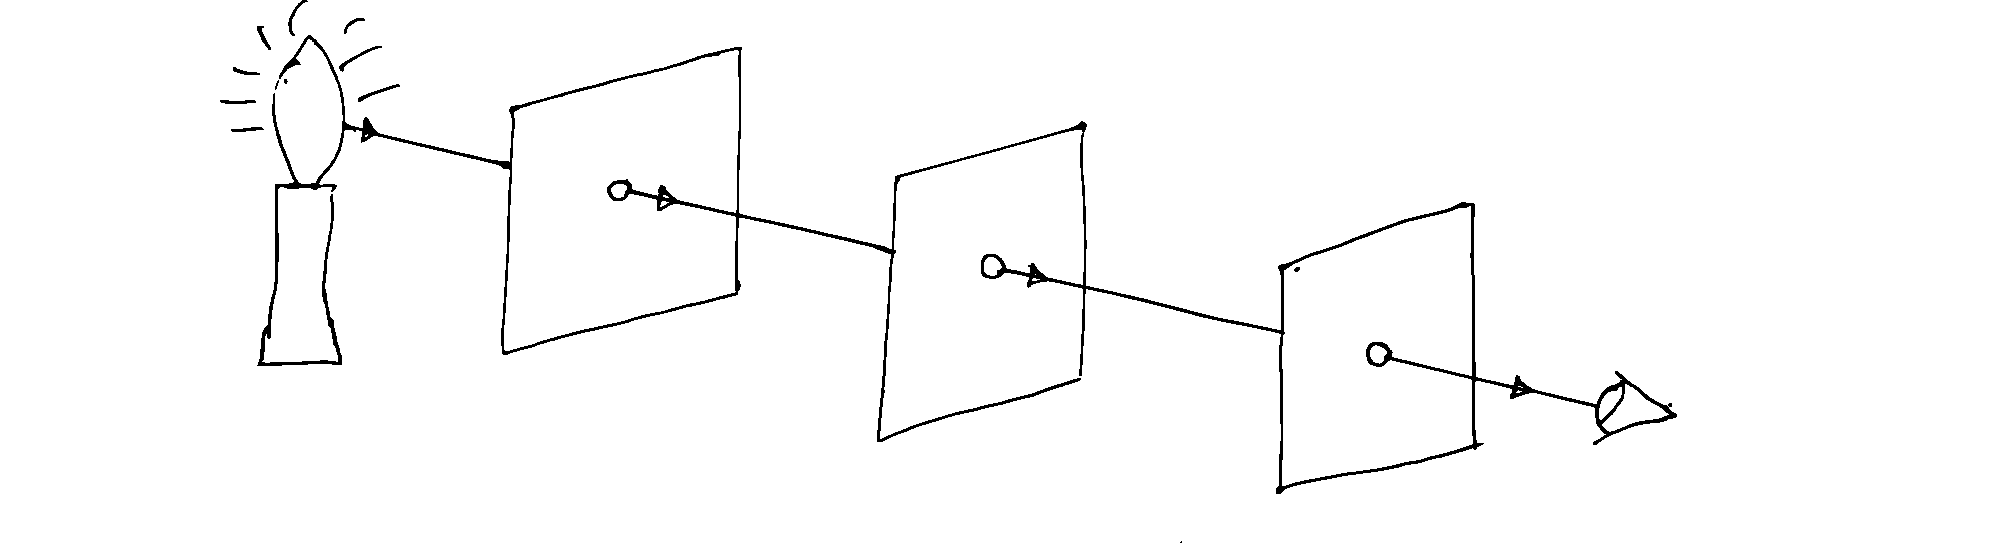
\includegraphics{./img/prop-of-light.png}
\caption{Experiment to show that light travels in straight lines}
\label{fig:prop-of-light}
\end{center}
\end{figure}

\subsubsection*{Activity Procedure}
\begin{enumerate}
\item{Arrange the cardboard pieces in between two books so they stand upright and arrange them in a straight line. The cardboard pieces should be at least 45 cm apart so that the holes are aligned.} 
\item{Place a light source 30 cm from the first piece of cardboard. Have an observer stand at the other end of the table.} 
\item{Look through the series of holes to see the light source.}
\item{Slightly displace one of the pieces of cardboard and again look through the holes.}
\end{enumerate}

\subsubsection*{Clean Up Procedure}
Collect all the used materials, cleaning and storing items that will be used later.

\subsubsection*{Discussion Questions}
\begin{enumerate}
\item{What does this experiment show about the way that light travels?}
\item{Draw a ray diagram to show the two alignments of the cardboard pieces.}
\end{enumerate}

\subsubsection*{Notes}
This activity is best done at night or in a dark room so that the light can be seen clearly through the holes.


%\subsection{Pinhole Camera}
%\begin{itemize}
%\item{Preparation Time: half hour}
%\item{Materials: Cardboard box, black paint if necessary, translucent screen (tissue paper, color gel, etc.), pin, tape, scissors, light source, any object}
%\item{Procedure: Cut out one side of the cardboard box and paint the inside black. Replace the cutout side of the box with your translucent screen, taping it shut along all four edges. On the opposite side of the box from the screen, poke a small hole with the pin. Your camera is now complete.\\
%In a dark room, shine a bright light source on an object and aim the camera at it so that the light from the object passes through the pinhole to the screen. If the source is bright enough, the image should appear, upside down, on the screen. Play around with the object distance until you have a large, clear image on the screen. It is recommended to try this outside on a bright day, but you will need to cover the space between the camera and your head completely so that no light can enter.}
%\item{Theory: Light travels in a straight line, and so light from the top of the object will pass at an angle through the pinhole, appearing at the bottom of the screen on the other side. Alternately, light from the bottom of the object will appear at the top of the screen. A strong light source is needed because the aperture pinhole is small and will only admit a small amount of light.}
%\end{itemize}
%
%\begin{center}
%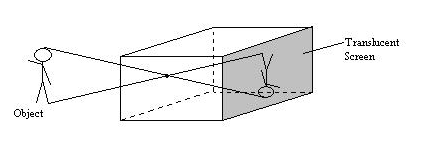
\includegraphics[width=8cm]{./img/pinhole-camera-1.png}
%\end{center}


\subsection{Pin Hole Camera}

\subsubsection*{Learning Objectives}
\begin{itemize}
\item{To construct a pinhole camera.}
\item{To use a pinhole camera to demonstrate that light travels in a straight line.}
\end{itemize}

\subsubsection*{Background Information}
Light rays travel in a straight line.  When the rays of light from a source pass through a small hole, the image of the source (any object producing or reflecting light) can be seen inverted on the other side of the hole.  A simple, closed box can be used to demonstrate this property of light.  This instrument is called a pinhole camera and it demonstrates the basis of photography.

\subsubsection*{Materials}
Cardboard box, plain paper, candle, kerosene, pin, glue, matches


\subsubsection*{Preparation Procedure}
\begin{enumerate}
\item{Remove one side of an empty box and on the opposite side make a small hole using a pin.} 
\item{Soak a piece of plain paper in kerosene to make it translucent.} 
\item{Using glue, cover the open side of the box with the translucent paper to act as a screen.} 
\item{Light the candle.} 
\end{enumerate}

\begin{figure}
\begin{center}
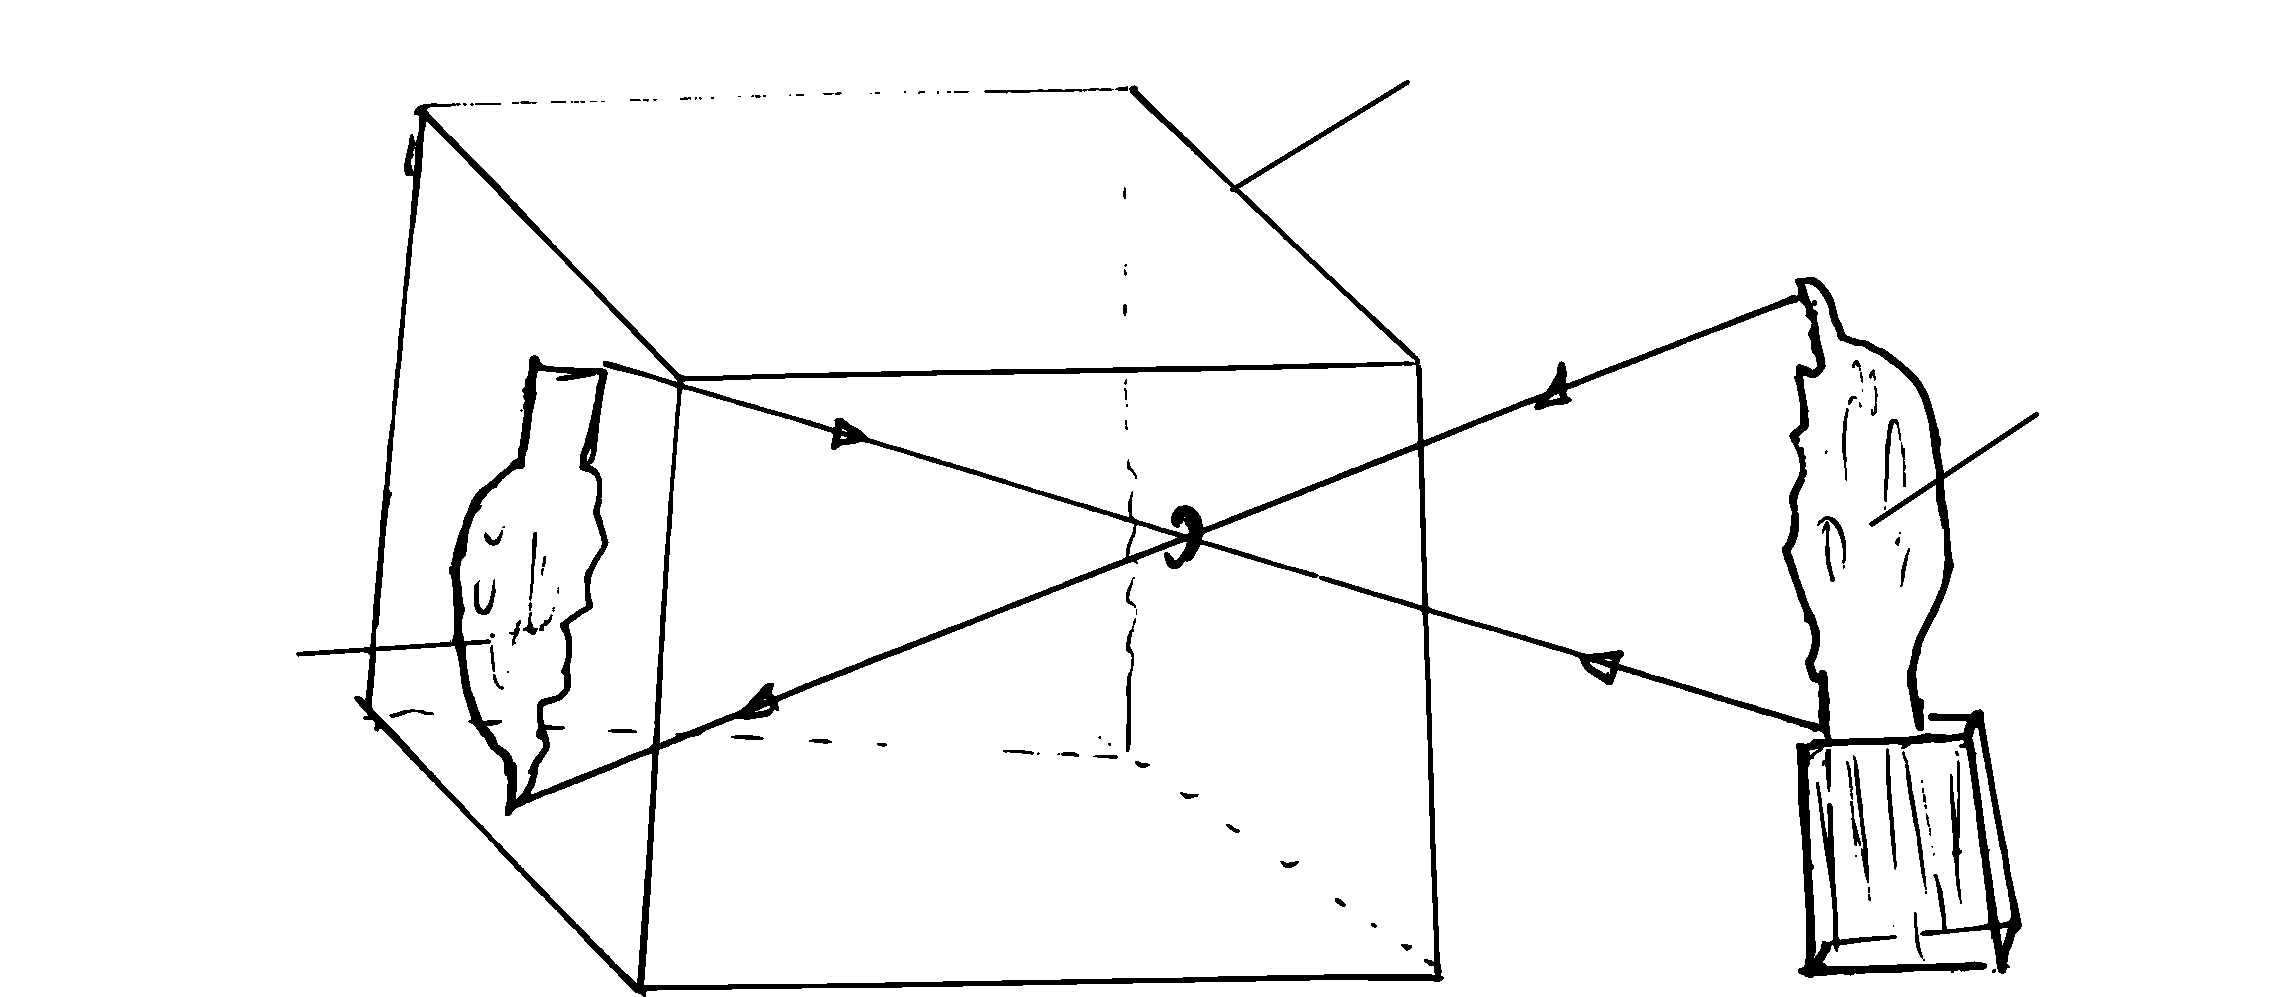
\includegraphics{./img/pinhole-camera.png}
\caption{Construction of a pinhole camera}
\label{fig:pinhole-camera}
\end{center}
\end{figure}

\subsubsection*{Activity Procedure}
\begin{enumerate}
\item{Place the candle in front of the box on the side with the small hole.} 
\item{Observe and record the image of the candle on the plain paper.} 
\end{enumerate}

\subsubsection*{Results and Conclusions}
Rays of light travel in a straight line. The observed image is inverted as the result of the path of light rays from the object to the paper -- the rays cross at the pin hole.

\subsubsection*{Clean Up Procedure}
The pinhole camera can be stored for later use.

\subsubsection*{Discussion Questions}
\begin{enumerate}
\item{What properties of light allow the image to appear?}
\item{Why is the image of the candle inverted?}
\item{Draw a ray diagram to represent how a pinhole camera works.}
\end{enumerate}

\subsubsection*{Notes}
The hole must be very small, clean for the pin hole camera to work properly. A large or jagged hole will create a blurred image.  
If it is difficult to see the image go to a darker room or try the experiment in the evening or night.


\subsection{Light through a Comb}
\begin{itemize}
\item{Preparation Time: 1 minute}
\item{Materials: comb, light source, optional mirror}
\item{Procedure: In a dark place, shine the light parallel to a table surface through the comb. The apertures in the comb will act as ‘beams’ of light. Reflect the beams off a mirror and observe the straight-line propagation of light.}
\item{Theory: Light travels in a straight line, even when reflected at a surface.}
\end{itemize}

	
	%Shadows
	
	
%Laws of Reflection (reflection of light)


\subsection{Laws of Reflection}

\subsubsection*{Learning Objectives}
\begin{itemize}
\item{To verify the laws of reflection in a plane mirror}
\end{itemize}

\subsubsection*{Materials}
Plane mirror, pins, thick cardboard, protractors and rulers, white paper, pen, pencil

\subsubsection{Activity Procedure}
\begin{enumerate}
\item{Place a plane mirror vertically on a sheet of white paper on top of the cardboard.}
\item{Draw a line along the back of the mirror.}
\item{Construct a perpendicular line to the line on which the mirror stands.}  
\item{Draw a line making an angle of incidence $i$ from the normal.}
\item{Insert two pins on the line drawn which makes an angle $i$ with the normal.}
\item{Look into the mirror such that the images of the pins look as if they are in straight line.}
\item{Insert two more pins so that they are in line with the images of the first two pins.  These two more pins mark the path of the reflected ray.}
\item{Remove the pins and draw lines joining the marks of the pins.}
\item{Using a protractor measure and record the angle between the reflected ray and the normal.}
\end{enumerate}

\subsubsection*{Results and Conclusions}
This practical is used to verify the Laws of Reflection and to observe and describe images formed in a plane mirror.  It will be seen that the angles of reflection are equal to the angles of incidence in each case.



%Applications (periscope, telescope)


\subsection{Kaleidoscope}
\begin{itemize}
\item{Preparation Time: 5 minutes}
\item{Materials: 3 or more mirrors of equal size OR 3 or more pieces of glass of equal size with metal foil on one side, tape; Optional: colored objects}
\item{Procedure: Tape the three mirrors together so that they form a triangular tube with the reflective sides facing in. Look through the kaleidoscope at any objects, especially colored beads or paper, and turn the scope to watch the pretty colors change!}
\end{itemize}